\documentclass[11pt,a4paper]{article}

\usepackage[utf8]{inputenc}
\usepackage[MeX]{polski}
\usepackage{graphicx}
\usepackage{wrapfig}
\usepackage{color}
\usepackage{amsmath}
\usepackage{amssymb}
\usepackage[inkscapelatex=false]{svg}
\usepackage{array, makecell}
\usepackage{mhchem}
\usepackage{tabularx}
\usepackage{braket}
\usepackage{pdfpages}

\usepackage{multicol}
\usepackage{colortbl}
\usepackage[Export]{adjustbox}
\adjustboxset{max size={0.9\linewidth}{0.9\paperheight}}
\usepackage[colorlinks=true,linkcolor=red,citecolor=green]{hyperref}

\textwidth=16cm
\textheight=23cm
\topmargin=-2cm
\oddsidemargin=0cm

\setlength{\parindent}{0em}
\setlength{\parskip}{0.6em}
\setlength{\jot}{12pt}

\renewcommand{\arraystretch}{1.4}
\renewcommand\theadfont{\bfseries}

\newcommand{\todo}[1]{\textcolor{red}{TODO: #1}}

\begin{document}

\title{MD - Symulacja Argonu}
\author{Dawid Karpiński}
\date{}
\maketitle

\section{Test stabilności programu}

\section{Kryształ}

\subsection{Topnienie kryształu}

\section{Gaz}

\subsection{Porównanie z gazem doskonałym}
Na koniec, porównano zależność ciśnienia od temperatury z danych symulacji do zależności teoretycznej:

$$
P(T) = \frac{3}{2} \frac{N k_B T}{V}
$$

\begin{figure}[ht!]
    \caption{\textbf{Porównanie zależności P(T) dla danych pomiarowych i gazu doskonałego}}
    \vspace{0.2cm}
    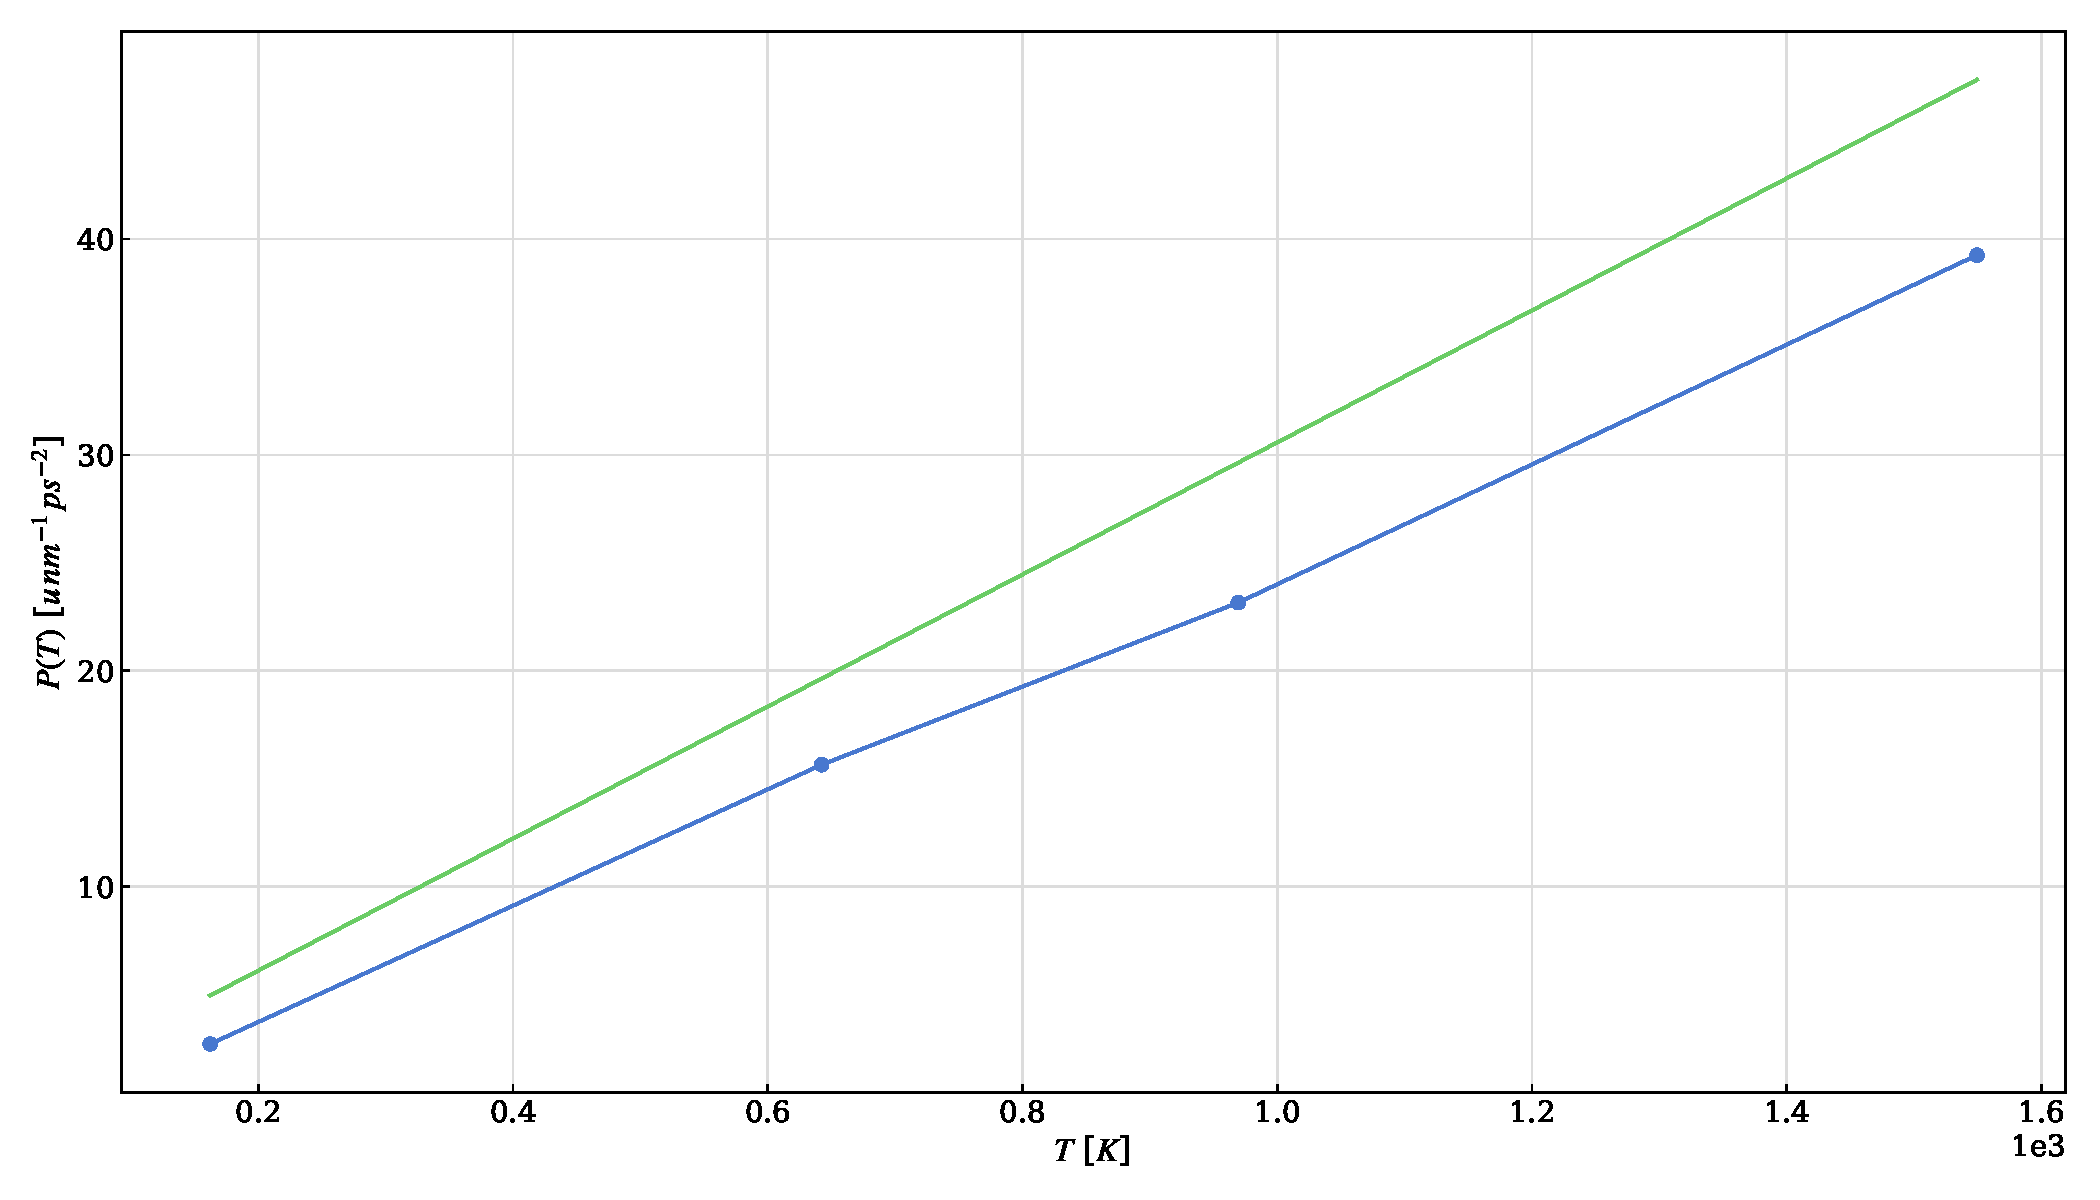
\includegraphics[width=\textwidth]{../figures/P_vs_T.pdf}
\end{figure}

hamiltonian od czasu
lub ciśnienie od czasu

\end{document}
